\documentclass[12pt,titlepage]{article}
\usepackage[spanish]{babel}
\usepackage[utf8]{inputenc}
\usepackage{amsfonts}
\usepackage{amsmath}
\usepackage{amssymb}
\usepackage{color}
\usepackage{graphicx} % para insertar imagenes
\usepackage{verbatim}
\usepackage{float}


\newcommand{\func}[2]{\texttt{#1}(#2)\\}
\newcommand{\tab}{\hspace*{2em}}
\newcommand{\FOR}{\textbf{for }}
\newcommand{\TO}{\textbf{ to }}
\newcommand{\IF}{\textbf{if }}
\newcommand{\WHILE}{\textbf{while }}
\newcommand{\THEN}{\textbf{then }}
\newcommand{\ELSE}{\textbf{else }}
\newcommand{\RET}{\textbf{return }}
\newcommand{\MOD}{\textbf{ \% }}
\newcommand{\OR}{\textbf{ or }}
\newcommand{\AND}{\textbf{ and }}
\newcommand{\tOde}[1]{\tab \small{O($#1$)}}
\newcommand{\Ode}[1]{O($#1$)}
\newcommand{\Thetade}[1]{{\small$\Theta$($#1$)}}
\newcommand{\Omegade}[1]{{\small$\Omega$($#1$)}}
\newcommand{\VSP}{\vspace*{3em}}
\newcommand{\Pa}{\vspace{5mm}}
\newenvironment{pseudo}{\begin{tabular}{p{11cm}l}}{\end{tabular}\VSP}

\newcommand{\gra}[1]{{\noindent\centering\includegraphics[width=14cm]{#1}}\\}

\title{{\sc\normalsize Algoritmos y estructuras de datos III}\\{\bf Trabajo Práctico Nº3}}
\author{\begin{tabular}{lcr}
De Sousa Bispo Mariano & 389/08 & marian\_sabianaa@hotmail.com \\
Grosso Daniel & 694/08 & dgrosso@gmail.com\\
Livorno Carla & 424/08 & carlalivorno@hotmail.com\\
Raffo Diego & 423/08 & enanodr@hotmail.com \\
\end{tabular}}
\date{\VSP \normalsize{Junio 2010}}
%\date{}
\begin{document}
\begin{titlepage}
\maketitle
\end{titlepage}
\tableofcontents
\newpage


	\begin{section}*{Introducción}	\addcontentsline{toc}{section}{Introducción}
		Este trabajo tiene como objetivo la aplicación de diferentes técnicas algorítmicas para la resolución de tres problemas particulares, el cálculo de complejidad teórica en el peor c aso de cada algoritmo implementado, y la posterior verificación empírica.
	
		El lenguaje utilizado para implementar los algoritmos de todos los problemas fue C/C++
	\end{section}


	\begin{section}{Situaciones de la vida real}
		El problema del Clique Máximo puede usarse como modelo para diversas situaciones de la vida real en ámbitos muy variados.\Pa
		
		\texttt{Aplicación Nº 1: }
			Por un lado tenemos los problemas que involucren personas (como nodos) y las relaciones entre ellos (los ejes) en distintas materias. Por ejemplo, puede ser útil para hacer promocionarse, dar productos gratis, y dado que el costo de cada producto puede ser elevado se trata de entregar la menor cantidad, asegurándose la máxima promoción posible. Podemos pedir que los ejes conecten a dos personas que trabajen juntas, y con esto seleccionar diversas empresas y repartir el producto a alguna persona de cada máximo clique de compañeros de trabajo de cada empresa, intentando con esto maximizar la promoción del producto en cuestión en cada empresa elegida.\Pa %CAPAZ HAYA QUE CAMBIARLO

%			Supongamos que una empresa de comptadoras quiere hacer propaganda de su producto. Para esto la empresa decide repartir computadoras gratis para que la gente las use en su trabajo, y dado su buen rendimiento, se promocione entre sus compañeros de trabajo. Como el producto no es barato de fabricar, esta empresa utilizaria una modificación de nuestro algorítmo para encontrar 

			%Otro ejemplo con personas como nodos, y "amistad" como ejes, podría usarse a la hora de formar una seleccion nacional en algún deporte de equipo. Una vez que el entrenador hace una selección preeliminar, para elejir entre ellos los que quedarían en el equipo se puede usar una modificacion del problema Max_Clique para saber cual es el mayor grupo de jugadores que se llevan bien entre si, lo que mejoraría el juego colectivo de dicha selección. (razon por la que riquelme no fue al mundial)
			
			%Podemos suponer que el Doctor Malito, némesis del conocido y carismático agente ingles Austin Powers, 
		\texttt{Aplicación Nº 2: }
			Un terrorista quiere infectar a la población con un virus. Supongamos que el virus es de transmición aérea, y dado el enorme costo de fabricación del virus, sólo se pudieron fabricar un par de cientos de ejemplares. El terrorista utilizaría una modificación de Max Clique para elegir sus blancos para que la probabilidad de contagio sea mayor. 
	\newpage
	\end{section}
	
	\begin{section}{Algoritmo exacto}
		\begin{subsection}{Explicación}
			El Algoritmo busca todas las formas de armar una clique utilizando la técnica de backtracking. Para esto, inicia la clique una vez desde cada vértice probando todas las combinaciones que lo incluyan, agregando vértices tal que forman un completo con los ya incluídos. Se necesita empezar una vez por cada nodo ya que la solución final podría no incluir el nodo inicial. De esta forma, se genera un árbol de backtracking teórico para cada vértice inicial. Mediante podas, evita recorrer el árbol por completo, siendo la solución final la máxima de las cliques encontradas. Como el algoritmo busca todas las cliques del grafo, la solución es la clique máxima del grafo.

		\begin{subsubsection}{Optimizaciones}
			Dado que se trata de un algoritmo de backtracking, la optimzación se basa en podar las ramas en las que estamos seguros que no va a aparecer el óptimo. Para esto tenemos que poder predecir, dado un estado actual, si es posible mejorar el óptimo encontrado hasta el momento.
			
			Por un lado, podamos las ramas que no forman un grafo completo, ya que no es solución.
			
			Por otro lado, evaluamos en cada paso del algoritmo la cantidad de vértices que falta explorar. Es decir, calculamos el tamaño de la clique máxima que podríamos formar considerando los vértices que ya estan incluídos en la solución actual. Si la cantidad de vértices que todavía no fueron evaluados más la cantidad de vértices ya pertenecientes a la clique actual es menor a la cantidad de vértices de la clique máxima encontrada hasta el momento, no tiene sentido seguir explorando esa rama ya que el tamaño de la clique máxima que se puede encontrar por ese camino es menor al tamaño de la máxima encontrada. Por este motivo, podamos esta rama.

			Además, para cada vértice que inicia la clique se intenta agregar los de mayor numeración tal que forman un completo. Por lo tanto, se evita repetir combinaciones. Supongamos que tenemos una clique de tres vértices, siendo estos el $<1,2,3>$. Con esta optimización, nunca han de analizarse los casos $<2,3,1>$; $<2,1,3>$; $<3,1,2>$ y $<3,2,1>$.
		\end{subsubsection}

		\end{subsection}
		\begin{subsection}{Detalles de la implementación}
			
			Almacenamos las relaciones entre los vértices en una matriz de $n \times n$, donde $n$ es la cantidad de vértices. Cada posición $(i,j)$ de la matriz contiene un $uno$ si existe la arista $(i,j)$ y un $cero$ en caso contrario. De esta forma se le asigna un número a cada vértice.\VSP

			A continuación, se muestra el pseudocódigo del algoritmo exacto.\\
			
			\begin{pseudo}
				\func{exacto}{matriz\_adyacencia,n}
				\tab $solucion \leftarrow \emptyset$\\
				\tab $\FOR i \TO n$\\
				\tab \tab buscar clique máxima desde el vértice $i$\\
				\tab \tab $\IF$ tiene más vértices que $solucion$\\
				\tab \tab \tab $solucion \leftarrow $ clique encontrada\\
				\RET $\#(solucion)$\\
			\end{pseudo}
			
			El algoritmo de backtracking recorre todos los vértices. Para cada uno de estos verifica si es adyacente con todos los vértices de la solución actual y si todavía no pertenece a la misma. Si es así lo agrega y repite este procedimiento (avanza). Si no, significa que recorrió todos los vértices y no logró formar una clique mayor a la encontrada, por lo que comienza a retroceder.

			Cuando retrocede, saca el último vértice $v$ que agregó a la solución y prosigue la búsqueda desde el vértice siguiente a $v$ en numeración. Si no hay un vértice que se pueda agregar, es decir, si ninguno de los siguientes forma una clique, el algoritmo sigue retrocediendo.
			
		\end{subsection}


		\newpage
		
		\begin{subsection}{Complejidad temporal}

		El algoritmo exacto utiliza la técnica de backtracking, con lo que genera un árbol donde cada rama es una posible solución, podando cuando considere que por ese camino no encuentra solución, o no encuentre una mejor a la actual.
		Dar la cota de complejidad de este algoritmo es complicado si tuviésemos en cuenta las podas que se realizan en el backtracking. Si quisieramos ajustar la cota, deberíamos buscar un grafo particular tal que las minimice (las podas), maximizando así la cantidad de vértices del árbol de backtracking.
		Por este motivo decidimos plantear un caso hipotético donde el árbol de backtracking se genere sin podas, verifícando para cada nodo $i$ las posibles cliques que lo contengan, intentando incluir sólo los de mayor numeración para no repetir soluciones. Como dijimos, esto es un caso hipotético, donde el algoritmo tiene un comportamiento menos eficiente que el real, y de esta forma conseguimos una cota superior poco ajustada, pero que a los fines prácticos nos da una idea de que aún en el peor caso, el algoritmo será más eficiente respecto a la cota calculada. 

		De esta forma el algoritmo verifica para cada vértice $i$, con $0 < i < n$, las cliques posibles que lo contengan, es decir, todas las combinaciones que tengan a $i$ más otros vértices entre $i$ y $n$ tal que forman una clique.

		Así, para cada vértice $i$ genera un árbol donde cada rama representa una clique que lo incluye, por lo que tendremos un árbol de $n-i$ factorial vértices.

		Como este procedimiento se repite con $i$ desde 1 hasta $n$ nos queda planteada la siguiente sumatoria: $\sum_{i=1}^{n}{i!}$ = $1! + 2! + 3! + ... + n!$

		Entonces la complejidad viene dada por: \Ode{1! + 2! + 3! + ... + n!}= \Ode{max(1!,2!,3!,...,n!)}= \Ode{n!}
		
		
		\end{subsection}
\end{section}



	\newpage

	\begin{section}{Heurística constructiva}
		\begin{subsection}{Explicación}
			Como Primera Heurística, en este caso constructiva, desarrollamos un algoritmo goloso para resolver el problema \texttt{MAX-CLIQUE} de manera aproximada.
			
			El mismo funciona de la siguiente manera:

			Sea $grados$ un arreglo de tamaño $n$, donde $n$ es la cantidad de vértices del grafo. En cada posición $j\; \forall 	1\leq j \leq n$ del arreglo está el grado correspondiente al vértice $j$.
			Para construir una clique ordenamos $grados$ en forma decreciente. El primer vértice del arreglo, es decir, el de mayor grado del grafo se considera parte de la solución final del algoritmo.
			Para completar la clique recorremos $grados$ en forma completa, y cada vértice que forma un completo con la solución parcial se agrega a la misma.
			Al terminar de recorrer $grados$ el algoritmo termina siendo la solución parcial, el resultado final.

			Al ser un algoritmo goloso, en este problema como en tantos otros, no devuelve necesariamente el óptimo. Particularmente, la clique está condicionada al vértice de mayor grado, y no necesariamente la solución óptima lo contiene.\VSP
		\end{subsection}
		\begin{subsection}{Detalles de la implementación}
			A continuación, se muestra el pseudocódigo del algoritmo de heurística constructiva.\\

			\begin{pseudo}
				\func{constructivo}{matriz\_adyacencia,n}
				\tab $grados[n] \leftarrow ordenar\_grados(matriz\_adyacencia)$\\
				\tab $solucion[n]$\\
				\tab $solucion[0] \leftarrow grados[0]$\\
				\tab $tamanyo \leftarrow 1$\\
				\tab $\FOR i \TO n$\\
				\tab \tab $\IF \neg solucion[i]$\\
				\tab \tab \tab $completo \leftarrow forma\_completo(solucion,i,matriz\_adyacencia)$\\
				\tab \tab \tab $\IF completo$\\
				\tab \tab \tab \tab $solucion[i] \leftarrow true$\\
				\tab \tab \tab \tab $tamanyo \leftarrow tamanyo + 1$\\
				\RET $tamanyo$\\
			\end{pseudo}

			\begin{itemize}
				\item \texttt{ordenar\_grados: } En la implementación, el arreglo $grados$ es de tipo tupla donde la primer componente representa el vértice y la segunda el grado. Dicho arreglo está ordenado según la segunda componente en forma decreciente. Lo ordenamos con el algoritmo de Quick Sort de $STL$.
				
					Para setear el grado de un vértice $i$ tenemos un contador inicializado en $cero$. Recorremos la columna de la matriz de adyacencia correspondiente a dicho vértice e incrementamos el contador por cada posición $(i,j)$ igual $uno$.
				\item \texttt{forma\_completo: } Para saber si agregar un vértice $v$ determina una solución al problema debemos verificar que forme un completo con los vértices ya incluídos. Para esto recorremos todos los vértices del grafo y para cada uno que pertenezca a la solución parcial chequeamos que sea adyacente a $v$. Si esto ocurre podemos agregar el vértice $v$ y agrandar la clique.
			\end{itemize}
		\end{subsection}
		\begin{subsection}{Complejidad temporal}
			El algoritmo empieza inicializando el arreglo $grados$ lo que tiene un costo de $n^2$ ya que para cada vértice recorre la columna correspondiente en la matriz de adyacencia (diseñada como un arreglo de arreglos).
			
			Como mencionamos anteriormente, $grados$ es ordenado con un algoritmo de QuickSort dado por la librería estándar de C++. El costo del algoritmo es CUADRATICO APARENTEMENTE, OJO AHI LA VIDA FIJATE Q DICE LA STL.
			
			El algoritmo constructivo, una vez realizadas las operaciones antes mencionadas, entra a un ciclo $for$ que itera desde $0$ hasta $n$. En cada iteración, debe en primera instancia, analizar una guarda $if$. De ser $falsa$, procederá a la siguiente iteración del ciclo (teniendo así costo constante). De ser $verdadera$ (es decir, el vértice $i$ no forma parte de la solución parcial), analizará si puede formar una nueva clique mayor, ahora con el vértice $i$ (en nuestro pseudo-código, la función $forma\_completo$ es la encargada de analizarlo). Con el resultado de $forma\_completo$ la iteración del $for$ principal analiza una guarda $if$ más de costo constante (en el peor caso realiza dos asignaciones y una suma). Sabemos entonces que el costo de este ciclo será como mínimo $n$. Analizaremos a continuación el costo de $forma\_completo$, para concluir el costo total del algoritmo.
			
			$forma\_completo$, como ya dijimos antes, recorre todos los vértices del grafo analizando que, los vértices que pertenecen a la solución parcial, sean adyacentes al que queremos agregar. Esta función itera por todos los vértices del grafo, teniendo así un costo lineal a la cantidad de vértices.
			
			Como el ciclo $for$ del algoritmo constructivo, en el peor caso, llamaría una vez por cada una de las $n$ iteraciones a la función $forma\_completo$, el costo del ciclo entonces es cuadrático a la cantidad de vértices.
			
			Tenemos entonces en el algoritmo constructivo, la inicialización del arreglo con costo de $n^2$, el QuickSort de STL, costo AOISJDOAISJD$N^2$ y el ciclo $for$ también con costo a lo sumo cuadrático. La complejidad asintótica del problema viene dada entonces por la suma de las complejidades anteriormente descriptas. Podemos afirmar que el costo es \Ode($n^2$), ya que \Ode($n^2 + n^2 + n^2$) = \Ode($3*n^2$) = \Ode($n^2$).
			
		\end{subsection}

\end{section}



	\newpage

	\begin{section}{Busqueda local}
		\begin{subsection}{Explicación}
			La heurística de busqueda local actua a partir de una solución inicial $S$, en este caso, a partir de la solución dada por la heurística constructiva. El algoritmo busca en la vecindad de la solución dada, $N(S)$, una solución mejor que ésta. Si no encuentra ninguna mejor, nos encontramos en un óptimo local (de la vecindad) que tomamos como solución del algoritmo.
			La vecindad $N(S)$ que elegimos en este problema es el conjunto de soluciones tales que no tienen uno y sólo uno de los vértices pertenecientes a $S$, es decir, $S \setminus \{v\} \cup L$ donde $L$ es un conjunto de vértices tal que $u \in L \Longleftrightarrow S \setminus \{v\} \cup \{u\}$ forma un completo.

			Para revisar la vecindad, sacamos un nodo de la solución óptima actual e intentamos agregar los vértices que no pertenecen a la clique. Luego, comparamos el tamaño de la clique que logramos contruir de esta manera con el tamaño de la clique correspondiente a la mejor solución vista de la vecindad. Si esta nueva solución es mejor, es decir, el tamaño de la clique es mayor al tamaño de la actual (mejor de la vecindad), dicha solución pasa a ser la mejor de la vecindad. Una vez revisada toda la vecindad comparamos la mejor solución encontrada en dicha vecindad con la mejor solución encontrada hasta el momento. Si es mejor, actualizamos el óptimo actual.
		\end{subsection}
		\begin{subsection}{Detalles de la implementación}
			A continuación, se muestra el pseudocódigo del algoritmo de heurística de búsqueda local.\\

			\begin{pseudo}
				\func{busqueda\_local}{solucion,tamanyo,matriz\_adyacencia,n}
				\tab $\IF tamanyo==1 \OR tamanyo==n$
				\tab \tab $\RET tamanyo$
				\tab $grados[n] \leftarrow ordenar\_grados(matriz\_adyacencia)$\\
				\tab $inicializar\_estructuras$\\
				\tab $\WHILE mejore$\\
				\tab \tab $\FOR j \TO n$\\
				\tab \tab \tab $sacar\_de\_clique(actual,i)$\\
				\tab \tab \tab $agrandar\_clique(actual,matriz\_adyacencia)$\\
				\tab \tab \tab$\IF tam\_actual>tam\_mejor\_vecindad$\\
				\tab \tab \tab \tab $actualizar\_mejor\_vecindad$\\
				\tab \tab \tab$\ELSE$\\
				\tab \tab \tab \tab $reconstruir(actual)$\\
				\tab \tab \IF $tam\_mejor\_vecindad>tamanyo$\\
				\tab \tab \tab $mejore$\\
				\tab \tab \tab $actualizar\_solucion$\\
				\RET $tamanyo$\\
			\end{pseudo}

		La primer cláusula \texttt{if} verifica si la solución constructiva encontró la clique tanto completa como la de un elemento. En ambos casos no tiene sentido aplicar la búsqueda local ya que, si encontró el completo, esta solución no podrá ser mejorada, al contener todos los vértices. Si sólo encontró un vértice, implica que el de grado mayor en el grafo es de grado cero, por lo tanto, todos sus vértices son de grado cero. 

		\begin{itemize}
			\item \texttt{inicializar\_estructuras:} Consiste en hacer dos copias de la solución, una para mejor vecindad y otra para actual, y setear dos variables que representan el tamaño de la clique de cada uno de los arreglos.
		
			\item \texttt{sacar\_de\_clique:} Esta función setea en $falso$ la posición $i$ del arreglo $actual$, es decir, excluye el vértice $i$ de la solución actual. Además, decrementa el tamaño de la clique, variable $tam\_actual$ y resetea una variable $nodo$ que indica si despues logra agregar algún vértice, esto sirve para reconstruir la solución en caso de ser necesario (conseguir un tamaño de clique igual al tamaño de la clique desde la que partió).
			
			\item \texttt{agrandar\_clique:} Esta función se encarga de buscar entre los vértices que actualmente no pertenecen a la clique e intenta agregarlos (agrega todo vértice que forma un completo con los ya pertenecientes), con el objeto de conseguir una de tamaño mayor. Por otro lado, setea $nodo$ con el valor del último vértice que agrega.

			\item \texttt{reconstruir:} En el caso donde el tamaño de la clique que logro contruir es igual al tamaño de la clique inicial, como queremos obtener el mejor de la vecindad, reconstruimos la clique anterior y continuamos, es decir, eliminamos $nodo$ y volvemos a agregar $i$.
			
			\item \texttt{actualizar\_mejor\_vecindad y actualizar\_solucion:} al encontrar una solución que es mejor a la que el algoritmo posee hasta ese momento, dependiendo del caso, la salva en uno de estos dos arreglos ($mejor\_vecindad$ o $actual$).
			
		\end{itemize}
		\end{subsection}
		\begin{subsection}{Desventajas}
		
		El algoritmo es estrictamente dependiente de la numeración inicial de los vértices. Para nodos de igual grado, al ordenarlos tiene prioridad el de menor numeración.
		Sea el siguiente gráfico, un ejemplo en el que esto sucede:
		
		
		PONER EJEMPLINGUI QUE NO ANDABAAAAAA era un caso de 7 nodoss q se qda con dos vertices en vez de tres.


		La clique dada por la heurística constructiva es el <1,2>.
		Cuando el algoritmo (búsqueda local) saca el vértice $uno$ de la clique, se mueve a la clique <2,4> ya que todos sus adyacentes tienen grado dos y el cuatro es el de menor numeración. Como no logra mejorar (no encuentra una clique que posea al dos y al cuatro, y además algún otro nodo), vuelve a la inicial de <1,2>. Prueba entonces sacando el dos, sin poder mejorar. Por lo tanto, la solución final es la que viene dada por el algortimo constructivo.
		
		\end{subsection}
		\begin{subsection}{Complejidad temporal}
			En un pricipio el algoritmo inicializa el arreglo de los $grados$ y lo ordena aplicando QuickSort, lo que tiene un costo de $n^2$. Luego, obtiene la solución inicial mediante la heurística constructiva que como ya vimos tiene también un costo de $n^2$ e inicializa los arreglos $actual$ y $mejor\_vecindad$ con costo lineal.

			La función $sacar\_de\_clique$ y $reconstruir$ tienen costo constante ya que consta sólo de indexaciones, asignaciones y otras operaciones elementales.

			La función $agrandar\_clique$ tiene costo $n^2$ porque recorre todos los vértices y para cada uno de los que todavía no pertenece a la clique, verifica si puede agregarlo. Para esto, recorre nuevamente todos los vértices y corrobora que sea adyacente a cada uno de los pertenecientes a la clique.

			La complejidad final del algoritmo es $n^4$ porque el ciclo \texttt{while} itera a lo sumo $n$ veces (la solución final puede verse mejorada a lo sumo $n$ veces) y por cada una de estas el ciclo \texttt{for} itera exactamente $n$ veces. En cada iteración del \texttt{for} hay una llamada a la función $sacar\_de\_clique$ y $agrandar\_clique$ las cuales tienen un costo de $n^2$. Eventualmente hay una llamada a $reconstruir$ lo que no altera la complejidad, ya que su costo es constante.
			
			El costo lineal en función de la cantidad de vértices del ciclo \texttt{while} está acotado por el caso hipotético de comenzar por una clique trivial, y en cada iteración, aumentar la clique en uno. Esto no puede pasar ya que se trataría de un grafo completo, que el algoritmo constructivo encontraría. En ese caso, el algoritmo termina antes de la primera iteración del \texttt{while}.
		\end{subsection}
\end{section}




	
	\newpage
	
	\begin{section}{Tabu-Search}
	\begin{subsection}{Explicación}
		Finalmente implementamos una metaheuristica, es decir, una heurística que guía otra heurística, en este caso la búsqueda local del ejercicio anterior.

		El \texttt{Tabu-Search} permite evitar que la heurística de búsqueda local se estanque en óptimos locales cuando en realidad fuera de la vecindad existía una solución óptima global (mejor que la local).
		Para lograrlo, permite al algoritmo perseguir una solución peor que la mejor obtenida mediante búsqueda local, por una cantidad máxima de iteraciones.
		Pasada esta cantidad, con-\\sideramos que el algoritmo ya buscó lo suficiente y la mejor solución encontrada hasta el momento debe ser la óptima.

		Para no revisar las vecindades que se revisaron anteriormente (que son muy cercanas a la vecindad actual),
		cada vez que decidimos movernos a otra vecindad porque tenemos un nuevo aspirante a óptimo (más allá de que sea peor que la mejor solución que encontramos hasta el momento, pero lo llamamos así por su similitud con el mismo en la búsqueda local)
		prohibimos revertir el cambio que hicimos para llegar del aspirante anterior al nuevo, o sea, prohibimos volver a agregar el vértice que sacamos.
		
		Cada vez que logramos mejorar, es decir, encontramos una clique de tamaño mayor a la máxima clique vista hasta el momento actualizamos la solución.
		Repetimos este procedimiento hasta agotar la máxima cantidad de iteraciones permitidas sin mejorar. Una vez que ocurre esto, el algoritmo termina, siendo la solución final la solución actual, es decir, la clique de mayor tamaño que logro encontrar.(Figura \ref{fig:seguimiento_busqueda_tabu})

			% --- Figura seguimiento algoritmo constructivo ---
			\begin{figure}[H]
				\centering
		    	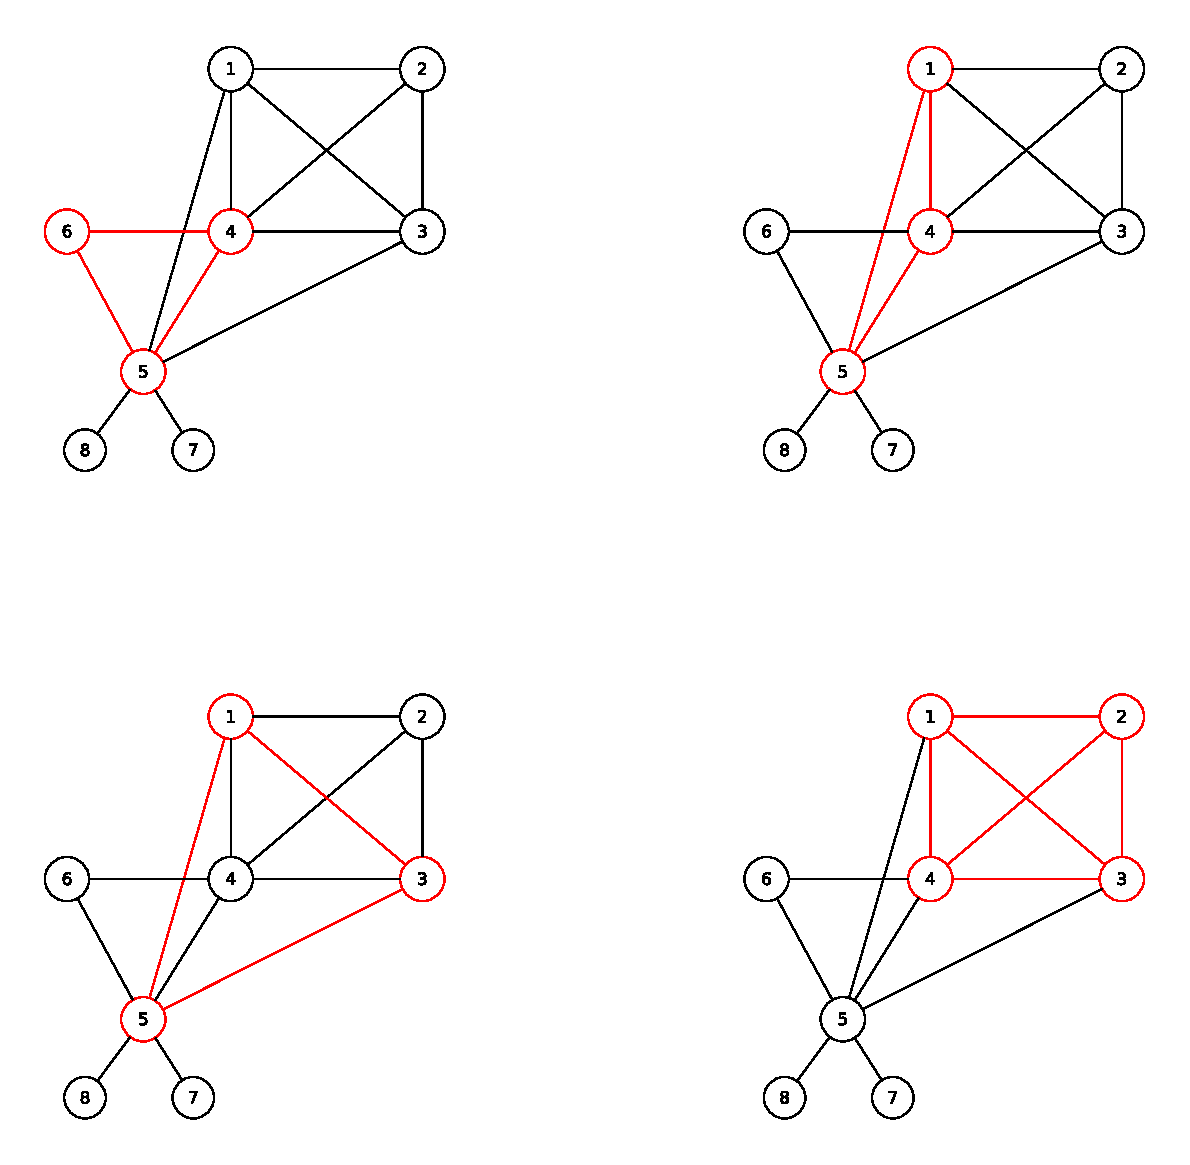
\includegraphics[scale=0.5]{tabu_search/seguimiento.eps}
			    \caption{Ejemplo de la heurística de búsqueda tabú}
			    \label{fig:seguimiento_busqueda_tabu}
			\end{figure}

		El seguimiento del algoritmo no está completo, se incluye sólo la parte más relevante (la rotación en la que se mejora la solución parcial).

		La heurística de búsqueda local nos da la clique formada por $<4,5,6>$. En una de las rotaciones, saca el vértice $cinco$ intentando formar una clique de mayor tamaño con $<4,6>$, al no poder hacerlo, retira el $seis$ (es decir, ahora el $seis$ y el $cinco$ son tabú). Es entonces que encuentra una nueva clique de cuatro nodos y actualiza la solución parcial con esta. El algoritmo continúa haciendo rotaciones sobre la nueva solución intentando agrandar la clique durante la cantidad de iteraciones permitidas y volviendo a permitir agregar los vértices tabú después de pasada su cantidad de iteraciones tabú. En este grafo en particular, no logra ninguna nueva mejora, siendo la clique observada en el último grafo de la figura, la solución que devuelve el algoritmo, así como el óptimo.



		\begin{comment}
		Esto lo implementamos mediante un arreglo de vértices (los índices representan los vértices), donde para cada uno guardamos la cantidad de iteraciones que falta para que deje de ser tabú (el algoritmo lleva la cuenta de las iteraciones).
		Luego, cuando revisamos las vecindades de un aspirante, evitamos aquellas donde la modificación implica agregar un vértice tabú.

		Los parámetros que indican cuanto tiempo una variable queda tabú y cuantas veces se puede iterar sin encontrar un nuevo óptimo antes de cortar el algoritmo, los buscamos empíricamente viendo los resultados obtenidos con distintos parámetros, y son bla y bla respectivamente.
		CAMBIAR LOS PARAMETROS!!!
		\end{comment}
	\end{subsection}
	\begin{subsection}{Detalles de la implementación}
		Almacenamos las relaciones entre los vértices en una matriz de $n \times n$, donde $n$ es la cantidad de vértices. Cada posición $(i,j)$ de la matriz contiene un $uno$ si existe la arista $(i,j)$ y un $cero$ en caso contrario. De esta forma se le asigna un número a cada vértice.\VSP

		A continuación, se muestra el pseudocódigo de la heurística de búsqueda tabú.\\

		Sea $n$ la cantidad de vértices del grafo.

		\begin{pseudo}
			\func{busqueda\_tabu}{solucion,tamanyo,matriz\_adyacencia}
			\tab $\IF tamanyo==1 \OR tamanyo==n$\\
			\tab \tab $\RET tamanyo$\\
			\tab $grados[n] \leftarrow ordenar\_grados(matriz\_adyacencia)$\\
			\tab $\WHILE mejore$\\
			\tab \tab $\FOR c \TO tamanyo$\\
			\tab \tab \tab $inicializar\_estructuras$\\
			\tab \tab \tab $rotar\_clique$\\
			\tab \tab \tab $\WHILE puedo\;seguir$\\
			\tab \tab \tab \tab $sacar\_de\_clique$\\
			\tab \tab \tab \tab $poner\_tabu$\\
			\tab \tab \tab \tab $formar\_completo(actual,matriz\_adyacencia)$\\
			\tab \tab \tab \tab $\IF tam\_actual>tamanyo$\\
			\tab \tab \tab \tab \tab $agrandar\_clique(actual,lista\_tabu)$
			\tab \tab \tab \tab \tab $actualizar\_solucion$
			\tab \tab \tab \tab \tab $c \leftarrow tamanyo$\\
			\tab \tab \tab \tab $\ELSE$\\
			\tab \tab \tab \tab \tab $restar\_tabu$\\
			\tab \RET $tamanyo$\\
		\end{pseudo}

		En la implementación mantenemos la solución actual tanto en una lista de vértices. La lista inicia ordenada de mayor a menor según los grados, esto lo hacemos para empezar a sacar desde el de menor grado ya que consideramos que es el que tiene más probabilidades de estar condicionando la clique. Además, tenemos un arreglo de tipo bool de tamaño $n$ donde el índice representa a los vértices y esta seteado en $verdadero$ si y sólo si el vértice pertenece a la clique actual. Mantenemos ambas estructuras porque usamos la lista para determinar el orden en que se eliminan (rotarla tiene costo constante) y el arreglo para verificar la pertenencia de un vértice a la clique (ya que esta operación en esta estructura de datos tiene costo constante).
		Por otro lado, mantenemos un arreglo de vértices (los índices representan los vértices), donde para cada uno guardamos la cantidad de iteraciones que falta para que deje de ser tabú una vez que son eliminados de la clique actual (el algoritmo lleva la cuenta de las iteraciones). Esto lo hacemos para no revertir los cambios recientemente hechos y cuando revisamos las vecindades de un aspirante, evitamos aquellas donde la modificación implica agregar un vértice tabú.

		La primer cláusula \texttt{if} verifica si la solución de búsqueda local encontró la clique tanto completa como la de un elemento. En ambos casos no tiene sentido aplicar el tabú search ya que, si encontró el completo, esta solución no podrá ser mejorada, al contener todos los vértices. Si sólo encontró un vértice, implica que el de grado mayor en el grafo es de grado cero, por lo tanto, todos sus vértices son de grado cero.

		El valor de verdad de la guarda del \texttt{while} $puedo\_seguir$ viene dado por la conjunción entre $tam\_actual \neq 1$, $\neg mejore$ e $iteracion<n$.
		Pedimos que el tamaño de la clique actual sea distinto de $uno$ ya que nos interesa movernos a soluciones vecinas. Si el tamaño es $uno$ en esa iteración saca el último vértice de la clique por lo que se pierde referencia a la misma moviéndose inmediatamente al primer vértice segun la numeración que no esté tabú.
		Por otro lado, el \texttt{while} itera mientras no logre mejorar para forzar la salida del ciclo cuando encuentre una clique de mayor tamaño que la actual y así empezar a sacar vértices desde la primer rotación (ya que también se fuerza la salida del \texttt{for}).
		La última condición es para asegurar la salida del ciclo, ya que podría no mejorar nunca y ciclar entre diferentes cliques. Además, esto determina la cantidad de iteraciones que le permitimos buscar sin lograr mejorar, es un parámetro que ajustamos de la siguiente manera AJUSTEMOSLO ALGUN DIAAAAAA!!!!!ukuyfuyjtjft5umj76fu7666m,6b,ib7,ki7k,i87fk7k,KUFMKUTJYTDMHYTMJUY6FMJUYMKY

		\begin{itemize}			
			\item \texttt{rotar\_clique: } Dado que fijar la pertenencia de un vértice a la clique condiciona el resultado final, el orden en que se eliminen los vértices puede hacer la diferencia entre un buen resultado y uno malo, a pesar de encontrar un buen criterio para hacerlo. Por este motivo, decidimos empezar eliminando de menor a mayor grado, y en cada iteración rotar la lista para sacar los vértices en otro orden.
			
			\item \texttt{sacar\_de\_clique: }Esta función saca de la lista el último elemento (el de menor grado entre los vértices con una misma 'antiguedad' en la clique) y setea en $falso$ la posición correspondiente en el arreglo (dejando tabú la operación inversa (agregarlo a la clique) tantas iteraciones como el tamaño de la clique con la que empieza a sacar), es decir, excluye el vértice de la solución actual. Además, decrementa la variable que indica el tamaño de la clique.

			LA CANTIDAD DE ITERACIONES QUE QUEDA TABU ES UN PARAMETRO ARREGLARLO
			
			\item \texttt{formar\_completo: } Esta función se encarga de buscar entre los vértices que actualmente no pertenecen a la clique e intenta agregarlos (agrega todo vértice que forma un completo con los ya pertenecientes), con el objeto de conseguir una de mayor tamaño. Para saber si agregarlo determina una solución al problema debemos verificar que forme un completo con los vértices ya incluídos. Para esto recorremos todos los vértices del grafo y para cada uno que pertenezca a la solución parcial chequeamos que sea adyacente al que pretendemos agregar. Si esto ocurre podemos agregarlo y agrandar la clique. Elegimos el vértice a agregar de mayor a menor grado.
			
			\texttt{Observaciones: }
			\begin{itemize}
				\item Al agregar condicionamos la clique resultante al igual que pasa al sacar sin hacer rotaciones (depende del orden en que lo hagamos la calidad de la solución). Es decir, encontrar una mejor solución depende del orden en que agreguemos los vértices, podriamos también hacer rotaciones para agregar pero esto aumentaría en $n$ la complejidad. Buscando un equilibrio entre eficiencia y calidad de la solución, decidimos que hacer ambas rotaciones (agregar, sacar) tenia una complejidad mayor a la que pretendemos aceptar, no hacer ninguno implica perdernos de encontrar mejores soluciones y obtener así soluciones muy precarias. Entonces elegimos arbitrariamente hacer las rotaciones sólo para sacar.

				\item Si el algoritmo vuelve a la solución inicial y todavía le restan iteraciones del \texttt{while} anidado, queremos evitar que repita exactamente el mismo procedimiento pasando nuevamente por soluciones ya visitadas por lo que forzamos la salida y aplicamos una rotación a dicha solución para explorar nuevas posibilidades.
			\end{itemize}

			\item \texttt{agrandar\_clique: } Esta función itera los vértices que están en la lista tabú e intenta agregarlos a la clique actual. Esto es porque como ya conseguí una solución mejor lograr agregar algún vértice que esta tabú contribuye aún más a la solución.

			\item \texttt{restar\_tabu: } Para cada vértice tal que tiene tabú mayor a $cero$ decrementa la cantidad de iteraciones que va a permanecer tabú. Si al decrementarlo deja de ser tabú lo elimina de $lista\_tabu$.

			Tanto en $formar\_completo$ como en $agrandar\_clique$ los vértices que agregamos a la lista de la clique actual los ponemos al principio de la misma, es una forma de poner tabú al menos tantas iteraciones como vértices había en la clique previo a agregarlos la operación inversa, sacarlos (ya que se saca siempre el último de la lista).
		\end{itemize}
	\end{subsection}

	\begin{subsection}{Desventajas}
		La numeración de los nodos toma un papel crucial a la hora de obtener una solución, es así que en casos patológicos puede pasar que:

		El algoritmo visite soluciones anteriormente exploradas ya que como se mueve constantemente de solución, puede eventualmente volver a la solución inicial (ejemplo: la búsqueda local nos da un clique de dos vértices que se encuentran en un ciclo, y este ciclo está unido a un completo de tres o más vértices). Si los vértices del completo tienen mayor numeración a los del ciclo, el algoritmo ciclaría tomando en cada iteración (mientras no se cumpla la restricción de iteraciones pasadas como parámetros) como solución dos de los vértices pertenecientes al ciclo, sin ver el completo.

		Para evitar pasar varias veces por las mismas soluciones, por cada iteración del \texttt{while} anidado se verifica si vuelve a la solución inicial, de ser así, se fuerza la salida y se procede a la siguiente rotación de la clique.
		A pesar de solucionar este problema para casos particulares como el que mencionamos (donde se parte de una solución y a través eliminar y agregar vértices se llega nuevamente a la solución inical), pueden existir casos donde se repitan soluciones desde distintas rotaciones de la clique inicial. Estos casos no son advertidos por el algoritmo.

		El siguiente seguimiento refleja el problema de la numeración (Figura \ref{fig:seguimiento_busqueda_tabu} y \ref{fig:seguimiento_busqueda_tabu_continuacion}).

			% --- Figura seguimiento algoritmo busqueda tabu ---
			\begin{figure}[H]
				\centering
		    	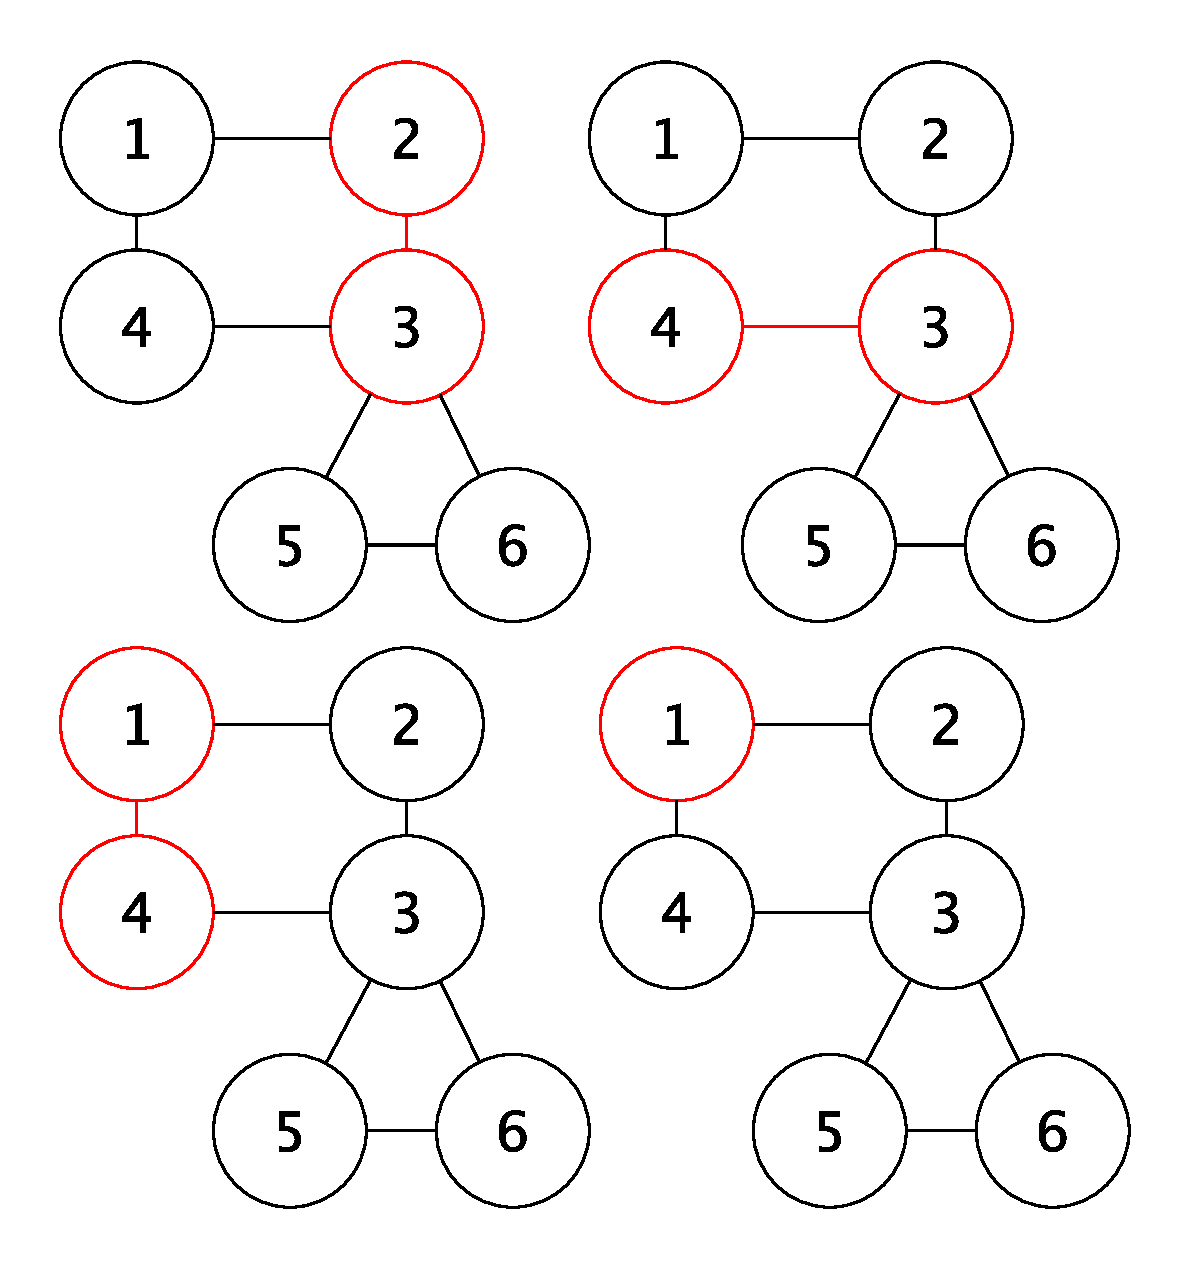
\includegraphics[scale=0.5]{tabu_search/segCasoMalo.eps}
			    \caption{Caso malo para la heurística de búsqueda tabú}
			    \label{fig:seguimiento_busqueda_tabu}
			\end{figure}

		En la primer rotación, el algoritmo al quitar el vértice $dos$ tiene dos caminos para seguir, o el $cuatro$ o el $cinco$. En el primero, se encontrará con un ciclo de cuatro nodos, sin poder agrandar la clique. En el segundo caso, encontrará una clique de tres, pudiendo mejorar y además encontrar el óptimo para este caso. Como ya dijimos, al tener dos vértices de igual grado, el algoritmo elige el de menor numeración, en este caso el $cuatro$. 

		Por lo tanto, en esta rotación, el algoritmo no puede encontrar la clique de tres.

			\begin{figure}[H]
				\centering
		    	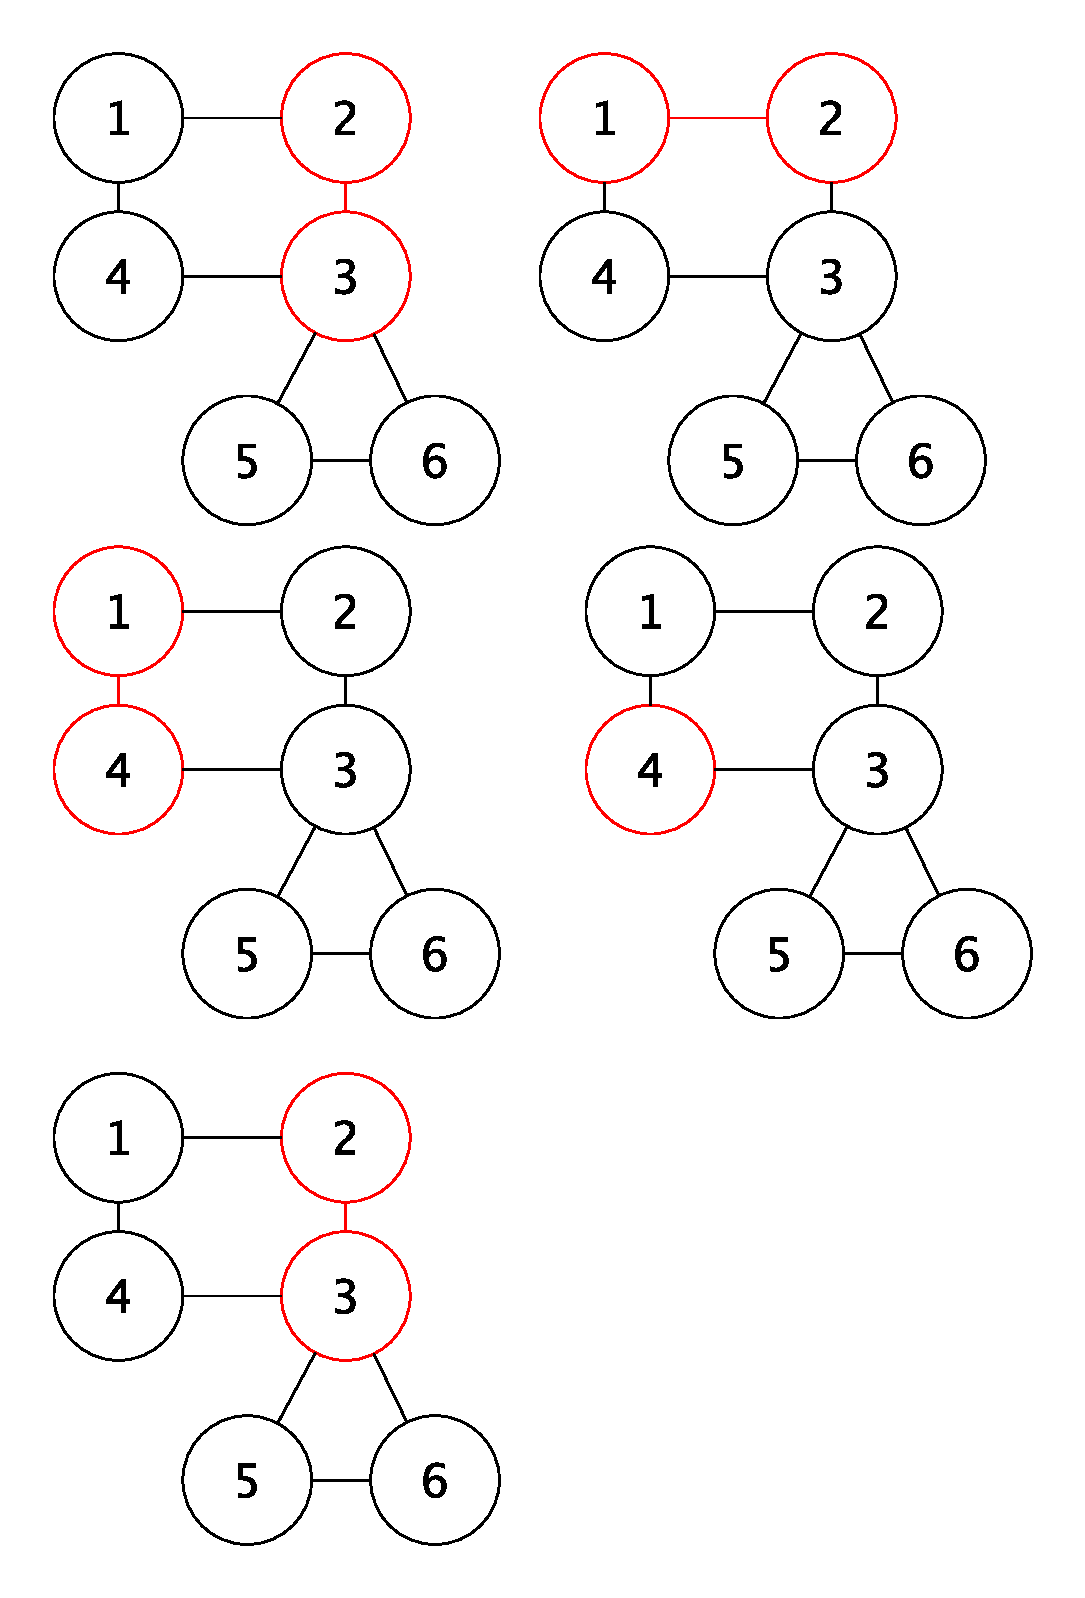
\includegraphics[scale=0.5]{tabu_search/segCasoMalo_cont.eps}
			    \caption{Caso malo para la heurística de búsqueda tabú}
			    \label{fig:seguimiento_busqueda_tabu_continuacion}
			\end{figure}

		En la segunda y última rotación, comienza por quitar el vértice $tres$, dejándolo tabú, y no pudiendo tomar otro vértice mas que el $uno$. Recorre el camino dado por los vértices $2,1,4$. Al llegar al $cuatro$, posee todos sus vértices adyacentes tabú, por lo que no puede seguir. Termina porque probó mejorar en todas sus rotaciones, sin poder lograrlo.

	\end{subsection}

	\begin{subsection}{Complejidad temporal}
			En un pricipio el algoritmo inicializa el arreglo de los $grados$ y lo ordena, lo que tiene un costo de $n^2$ ya que se utiliza el algoritmo de ordenamiento $QuickSort$. Luego, obtiene la solución inicial mediante la heurística de busqueda local que como ya vimos tiene un costo de $n^4$.

			La función $rotar\_clique$, $sacar\_de\_clique$ y $poner\_tabu$ tienen costo\\ constante ya que constan sólo de indexaciones, asignaciones y operaciones elementales sobre listas.

			La función $formar\_completo$ itera por todos los vértices y para cada uno de estos verifica si es factible agregarlo a la clique, lo cual tiene un costo de $n^2$ ya que dicha verificación consiste en recorrer todos los vertices del grafo y ver que el vértice que se pretende agregar es adyacente a cada uno de estos. Además, se concatena la lista de los vértices agregados con la lista de la clique actual lo que tiene un costo constante.

			La función $agrandar\_clique$ tiene costo $n^2$ ya que no es más que una llamada a la función $formar\_completo$ con todos los vértices permitidos, es decir, previo a la llamada se resetea el arreglo $tabu$.

			 La cantidad de iteraciones del primer ciclo \texttt{while} se puede acotar por $n$ (seria un caso hipotetico en el que la mejora sea sólo de un vértice, es decir, se inicie con la clique trivial (tamaño $uno$) y en cada iteración de este ciclo se logre incrementar en uno el tamaño de la clique). En cada una de estas iteraciones hay un ciclo \texttt{for} que se ejecuta a lo sumo tantas veces como el tamaño de la clique, también puede ser acotado por $n$, dentro de este ciclo se resetean las estructuras (la lista y los arreglos) lo que tiene un costo lineal. Además, hay un ciclo \texttt{while} (dentro del for) que se ejecuta a los sumo $n$ veces y en cada una de las iteraciones hay una llamada a la función $sacar\_de\_clique$ con costo constante y $formar\_completo$ con costo $n^2$, en caso de lograr mejorar hay una llamada a la función $agrandar\_clique$ con costo $n^2$, en caso contrario, hay una llamada a la función $restar\_tabu$ de costo lineal (recorre todos los vértices decrementando la cantidad de iteraciones que permaneceran tabú). Entonces la complejidad del \texttt{while} anidado es:  \Ode{n*(\Ode{sacar\_de\_clique} + \Ode{formar\_completo} + \Ode{agrandar\_clique} + \Ode{restar\_tabu})} = \Ode{n*(1+n^2+n^2+n)} = \Ode{n^3}.

			 Finalmente, se deduce que la complejidad final del algoritmo es $n^5$ ya que acotamos tanto la cantidad de iteraciones del cliclo \texttt{while} como del \texttt{for} por $n$, entonces tenemos \Ode{n*n*\Ode{while\_anidado}}=\Ode{n^5}.\Pa
			 
			 \texttt{Observación: } En la función $formar\_completo$ para ver si es factible agregar un vértice a la clique en vez de recorrer todos los vértices del grafo como hacemos, se podria sólo recorrer los vértices pertenecientes a la clique ya que están en una lista, pero la complejidad sería la misma y deberiamos ir agregando a la lista a medida que se decide agregar un vértice (para considerarlo en las proximas verificaciones) y esto no nos permite hacerlo en el orden deseado (ya que queremos agregar al principio de la lista de la clique actual de menor a mayor grado y los recorremos de mayor a menor grado). Como ya mencionamos esto no mejoraria la complejidad asintotica y aumentaria la complejidad de comprensión del código.
	\end{subsection}

\end{section}

	%	\begin{subsection}{Anexo}
		\begin{subsubsection}{Correctitud ejercicio 1}
		La siguiente tabla representa la correspondencia entre las variables de entrada ($b$ y $n$) en 
		cada iteración del algoritmo implementado:

		\vspace{0.5cm}
		\begin{center}
		\begin{tabular}{|l|c|c|c|c|c|}
			\hline
			iteración   & $1$ & $2$           & $3$             & ... & $k$ \\
			\hline
			$n$         & $n$ & $\frac{n}{2}$ & $\frac{n}{2^2}$ & ... & $\frac{n}{2^{k-1}}$ \\
			\hline
			$b$         & $b$ & $b^2$         & $b^4$           & ... & $b^{2^{k-1}}$ \\
			\hline
		\end{tabular}
		\end{center}

		\vspace{0.5cm}
		\noindent Sean \\
		\indent
		\begin{tabular}{lp{6cm}}
			$A_k = \frac{n}{2^{k-1}}$ & la sucesión con los valores de $n$ en la iteración $k$, y \\
			$Z_k = impar(A_k) * b^{2^{k-1}} + par( A_k )$ $^{[1]}$ & la sucesión que tiene los valores de $b$ corres\-pondientes a los $n$ impares y $1$ en los pares
		\end{tabular} \\
		\vspace{0.2cm}
		entonces el cálculo hecho por el algoritmo está dado por 
		$$\displaystyle\prod_{i=1}^k Z_i = b^n$$

		Luego de cada multiplicación toma módulo $n$ ya que
			$$b^k * b^{n-k}\; mod\;n = ((b^k\;mod\;n)*(b^{n-k}\;mod\;n))\;mod\;n\;\forall\;k\leq n ^{[2]}$$ 

		De esta manera, incluso si el cálculo de $b^n$ es un número tan grande que no entra en el 
		tamaño de la variable, se va a poder realizar sin problemas (suponiendo que $(n-1)^2$ entra 
		en una variable).


		\vspace{0.5cm}
		\noindent{\footnotesize [1] $par(x)=1-impar(x)$\\ $impar$ se define como:
		\begin{displaymath}
			impar(x)=\left\{
			\begin{array}{ll}
				1 & $si $x$ es impar$ \\
				0 & $sino$
			\end{array}\right.
		\end{displaymath}
		} \\
		\vspace{0.5cm}
		{\footnotesize [2] Por propiedades del módulo $x*y\; mod \; z = ((x\; mod\; z)*(y\; mod\; z))\;mod\; z$ } \\
		\end{subsubsection}
	\end{subsection}

	
	\newpage
	
	\begin{section}{Resultados}

		\begin{subsection}{Comparación de tiempos}

		En el siguiente gráfico se medirán todos los algoritmos implementados en función del tiempo. Las intancias analizadas varían en cantidad de vértices entre $uno$ y $cien$, siendo las aristas que los conectan aleatorias para todos los casos(Figura \ref{fig:Tiempo de los Algoritmos}).
		
		Queremos ver si en la ejecución empírica de estos programas, existe diferencia en cantidad de tiempo como esperamos debido a la diferencia de complejidad entre ellos.
		
		\begin{figure}[H]
			\centering
					\includegraphics[width=9cm,angle=-90]{conclusiones/heuris_vs_exacto.eps}
			\caption{Pruebas de tiempo de todos los Algoritmos implementados}
			\label{fig:Tiempo de los Algoritmos}
		\end{figure}
		
		Como esperabamos, y dada estas instancias, se nota que el costo en segundos del algoritmo exacto supera sin ninguna duda a cualquiera de las heúristicas a partir de los grafos de 50 vértices. Los casos son relativamente pequeños y la diferencia entre los algoritmos son importantísimas. Si bien la cantidad de segundos que al el exacto le toma calcular la solución para estos casos es pequeña (casi tres segundos en el peor caso para estas instancias), a medida que el tamaño de los grafos aumente, el tiempo crecerá también hasta volver impractible este algoritmo.

		Viendo las instancias calculadas por el algoritmo exacto, notamos algunas de ellas que tiene un comportamiento distinto al esperado, es decir, tardaron más de lo que tardaron tanto los casos predecesores como antecesores. Podemos atribuir este fenómeno a dos cosas:

			\begin{itemize}
				\item Al ser un cálculo de tiempo, y estar corriendo el algoritmo bajo un sistema operativo, no podemos afirmar que el tiempo reflejado en el gráfico sea puramente el costo de $exacto$ (es más podemos afirmarlo que no lo es, ya son sistemas multi-tareas, no podemos afirmar qué tiempo es el que le correspondió al algoritmo).
				\item El algoritmo pudo realizar para ese caso en particular y así tener que realizar mayor cantidad de cálculos, que son directamente proporcionales a la cantidad de tiempo.
			\end{itemize}

		Existen además, casos en los que el algoritmo (exacto), se comporta de manera más eficiente que lo esperado. Atribuímos esto a efectivas podas que favorecieron a mejorar el tiempo de corrida.

		Debido a la escala, no podemos afirmar que la complejidad que analizamos para las heúristicas sea correcta.\VSP

		Analizaremos en el siguiente gráfico, sólo las heurísticas, para ver si existen diferencias en el costo temporal entre cada una de ellas, se generaron aleatoriamente 100 instancias con $8x$ vértices, donde $x$ es el número de instancias.	
		
		\begin{figure}[H]
			\centering
					\includegraphics[width=9cm,angle=-90]{conclusiones/heuris.eps}
			\caption{Pruebas de tiempo de todas las Heurísticas implementadas}
			\label{fig:Tiempo de Heuristicas}
		\end{figure}
		
		Podemos ver en principio que existen diferencias entre el costo temporal de búsqueda tabú y constructiva/búsqueda local.
		
		La diferencia en costo (tiempo) entre estos algoritmos es significativa, resta ver entonces, si esa diferencia se hace merecer, al mejorar la calidad de la solución (Se tratará en 'Comparación de Calidad').
		
		No podemos considerar como $outliers$ ninguno de los puntos de tabú search que parecen alejarse de la curva, debido a que el algoritmo depende las iteraciones si mejora o no, y esto a su vez, depende del grafo en particular.
		
		No podemos afirmar por el momento que exista diferencias de tiempo entre la heurística constructiva, y la de búsqueda local. La diferencia de complejidad entre los algoritmos, dificulta su apreciación (debido a la escala en la que debe graficarse para incluir todos los puntos).\VSP
		
		En el siguiente gráfico, se incluirán sólo la heúristica de búqueda local y constructiva, con el objeto de denotar alguna diferencia en el coste temporal entre ellas. Se realizaron 50 intancias que varían el tamaño entre 500 y 1200 vértices de a múltiplos de 14, con grafos aleatorios.

		\begin{figure}[H]
			\centering
					\includegraphics[width=9cm,angle=-90]{conclusiones/heuris_rapidas2.eps}
			\caption{Pruebas de tiempo de Constructivo vs. Búsqueda Local [500-1200]}
			\label{fig:Tiempo de const_bus_loc}
		\end{figure}
		
		Podemos observar que recién a partir de grafos de 700 nodos empieza a existir diferencia significativa entre el tiempo que toma cada instancias para analizar con búsqueda local y con constructivo. Podemos concluir con eso que la búsqueda local es más conveniente para estos casos menores a 700 vértices, ya que podemos inclusive hasta mejorar la solución, sin perder tiempo considerable (recordar que búsqueda local comienza con el resultado de la constructiva y nunca lo empeora).\VSP
		
		Se incluye debajo, el gráfico con 100 instancias, entre 0 y 800 vértices (nuevamente grafos aleatorios). Los algoritmos que se muestran son el de búsqueda local y constructivo. El gráfico tiene como objetivo mostrar que no existen diferencias significativas en el costo temporal de ellos para intancias que se encuentren en esa franja de tamaño.
		
		\begin{figure}[H]
			\centering
					\includegraphics[width=9cm,angle=-90]{conclusiones/heuris_rapidas.eps}
			\caption{Pruebas de tiempo de Constructivo vs. Búsqueda Local [0-800]}
			\label{fig:Tiempo de const_bus_loc}
		\end{figure}

		\end{subsection}

		\begin{subsection}{Comparación de calidad}

		Para obtener conclusiones sobre la calidad de los algoritmos, realizamos trescientos grafos de tamaño cien con aristas aleatorias, los cuales fueron analizados por el algoritmo exacto y por todas las heurísticas previamente descriptas. Para moldear esta información en datos tangibles y posibles de analizar realizamos un histograma que en el eje $x$ tenga el tamaño de la clique encontrada, y en el eje $y$ la cantidad de instancias (para cada algoritmo) que se encontraron con esa clique. Si bien no nos da precisión en cuanto a qué casos fueron los que dieron 'igual' o 'peor' del óptimo, tenemos una idea general del comportamiento de todas las heurísticas y su aproximación al exacto (ya vimos que dependiendo del grafo, el comportamiento de las heurísticas puede variar significativamente).
		
		A continuación, se muestra el histograma con estos resultados.
		\begin{figure}[H]
			\centering
					\includegraphics[width=9cm,angle=-90]{conclusiones/calidad.eps}
			\caption{Pruebas de calidad de todos los Algoritmos implementados}
			\label{fig:Calidad de los Algoritmos}
		\end{figure}
		
		En la figura anterior podemos ver como el algorítmo de búsqueda tabú es el que más se aproxima al tamaño de la clique óptima dada por el algoritmo $exacto$. Es significativo el nivel de mejora de la búsqueda tabú en relación al resto (recordar que cada algoritmo parte de la solución dada por el predecesor en complejidad).
		
		Vemos también que el algoritmo de búsqueda local tiende a mejorar las soluciones dadas por el constructivo, es decir, para cliques de $seis$ o $siete$ encontró más casos constructivo que búsqueda local. En conclusión, como búqueda local parte de la solución dada por la constructiva y nunca la empeora, la diferencia que hay entre estos en las cliques de ocho y nueve, nos hacen inferir que búsqueda local, mejora en uno o dos vértices la solución dada por la heurística constructiva.
		
		Para estas instancias analizadas, también podemos inferir que el algoritmo constructivo encuentra cliques relativamente cercanas a la exacta, siempre menor o igual que búsqueda local o tabú teniendo en cuenta que su complejidad es mucho menor.
		
		Nuestro generador de grafos intenta generarlos de la forma mas aleatoria posible. De todas formas no hemos encontrado casos en donde constructivo dé el exacto (o si existen, son tan pocos que no se aprecian en el gráfico). Es interesante pensar que si el constructivo encuentra la clique máxima, esta no va a modificarse ni con búsqueda tabú ni con búsqueda local. Sería pertinente entonces, como criterio posible de decisión, encontrar la relación cantidad de aristas/cantidad de nodos, si esta relación se aproxima al completo o es muy chica (es decir hay muy pocas aristas), sería conveniente aplicar el algoritmo constructivo que en ambos casos, tiende a encontrar el óptimo (si hay un completo muy grande, muy posiblemente el de grado mayor esté incluído, al igual que si existen muy pocas aristas).
		\end{subsection}
	\end{section}

	\begin{section}{Conclusiones}
	\tab Luego de haber efectuado los análisis teóricos de complejidad y habiendo efectuado comparaciones en cuanto a la $performance$ y a la precisión de cada algoritmo, podemos sacar algunas conclusiones:
	\begin{itemize}
		\item El algoritmo $exacto$, como lo indica su nombre, es el único algoritmo que nos devuelve siempre la solución precisa al problema de la clique máxima. Sin embargo, el costo de operaciones y en tiempo del algoritmo es factorial, siendo su utilización para grafos grandes impracticable.
		\item El algoritmo de heurística constructiva es el algoritmo de heurística mas rápido que implementamos, y también el menos preciso en líneas generales. Su complejidad en cantidad de operaciones es cuadrática con respecto al tamaño del grafo. Como aproximación performante al problema de clique máxima es una buena elección, si bien como antes vimos, puede estar lejos de la óptima. Si el problema acepta una precisión no muy buena, pero requiere minimizar el tiempo de espera para obtener el resultado, $constructivo$ sería una buena opción
		\item La heurística de búsqueda local resulta ser más precisa que la heurística constructiva, elevando el orden de complejidad a \Ode{n^4}. En el análisis empírico, en las computadoras en las que fue corrido y para el tamaño de test en el que fue analizado, esta relación calidad/tiempo de ejecución nos pareció adecuada, ya que logramos mejores resultados y la resolución de los casos fue rápida.
		\item El algoritmo de heurística de búsqueda tabú, contiene la implementación más fina en la búsqueda de la clique máxima. La experimentanción sobre este algoritmo nos mostró la pequeña línea que existe entre 'tiempo de ejecución' y 'presición'. Si bien es clara la mejora que produce sobre los demás algoritmos, intentamos siempre mejorar los casos en los que esta heurística no funcionaba, en un intento por tender cada vez más al óptimo. Al tener una nueva idea sobre como mejorarlo, nos dabamos cuenta que la complejidad aumentaba como mínimo en un orden y el código se complicaba aún más. Durante los $tests$ realizados, vimos que la diferencia en el tiempo de ejecución entre este y el resto de los algoritmos, no era menor. 
	\end{itemize}
	En nuestra primera aproximación con los algoritmos heurísticos, podemos concluir que dependiendo del problema en particular, y qué esté uno dispuesto a perder en pos de una mejoría (tiempo o calidad) radica en la elección del algoritmo.

		\begin{subsection}{Evaluación de Problemas}
		\tab Al comenzar el informe se mencionaron dos situaciones que pueden ser modelados mediante grafos, más precisamente con un problema de clique máxima, veamos como nuestros algoritmos se relacionan con estas situaciones. 
			\begin{itemize}
			\item El primer problema consistía en la empresa que queria promocionar su producto, con lo que utilizaba el programa de max\_clique para determinar las cliques máximas de cada empresa elegida para promosionarse. Suponiendo que las empresas que eligió son multinacionales, con miles de empleados cada una, no creemos conveniente el uso del max\_clique exacto, ya que el tiempo de ejecución sería muy costoso, con lo cual debería optar por un algorimo heurístico. Con lo visto en las pruebas, dado el tamaño del grafo con el que modelaríamos el problema, optaríamos por el algorítmo de busqueda tabú, ya que para estos tamaños de entrada la diferencia de tiempo no es tan significativa en comparación a posible maximización de las ganancias.
			\item En el segundo problema, el terrorista se enfrenta a un gran problema, que es la enorme cantidad de personas en el planeta (aproximadamente 6.000.000.000 personas). Con esto se hace imposible aplicar un algoritmo exacto. Dependiendo de las carácteristicas del virus, este puede ser extremadamente contagioso, y suponiendo esto, tal vez no sea de tanta importancia que el clique de personas elegido sea el máximo. Consideramos que de el algoritmo de heurística constructiva podría dar buenos resultados ya que es tal vez el único algoritmo que terminaría en un tiempo aceptable, que puede ser de varios meses, y tiene una mayor probabilidad de contagio que simplemente eligir personas que se conozcan con mucha gente.
			\end{itemize}
		\end{subsection}
	
	\end{section}
	
	\begin{section}{Mediciones}
		Para contar la cantidad aproximada de operaciones definimos una variable inicializada en $cero$ la cual incrementamos luego de cada operación. En el código puede verse la llamada a la función \texttt{O(x)}, donde $x$ es un valor positivo entero, el cual es sumado a la cantidad de operaciones parcial para una vez terminado el algoritmo, poseer la cantidad de operaciones que realiza para una instancia dada.

		Se realizaron las mediciones de tiempo mediante una macro que cuenta ejecuta sucesivamente el algoritmo hasta que:
			\begin{itemize}
				\item Se cumple medio segundo y saca un promedio de los tiempos o,
				\item Una ejecución tarda más de medio segundo, dejando el valor de esa ejecución.
			\end{itemize}
	
	\end{section}
	\begin{section}{Compilación y ejecución de los programas}
	Para compilar los programas se puede usar el comando \texttt{make} (Requiere el compilador \texttt{g++}).
	
	Para correr todos los algoritmos, ejecute en terminal \texttt{./max\_clique.sh [nombre\_de\_archivo.in]} siendo los \texttt{nombre\_de\_archivoX.out} guardados en la carpeta $out$. ($tabu\_search$ se ejecutará con los parámetros que consideramos mejores en el análisis del algoritmo. No es necesario compilar los programas previamente).
		
	Se pueden correr los programas de cada ejercicio ejecutando \texttt{./exacto}, \texttt{./constructivo}, \texttt{./busqueda\_local} y \texttt{./tabu\_search} respectivamente. Los programas leen la entrada de stdin y escriben la respuesta en stdout. Para leer la entrada de un archivo \texttt{Tp3X.in} y escribir la respuesta en un archivo \texttt{Tp3X.out} ses puede usar:\\ \texttt{./(ejecutable) < Tp3X.in > Tp3X.out}

	Para contar la cantidad de operaciones: \texttt{./(ejecutable) count}. Devuelve para cada instancia el tamaño seguido de la cantidad de operaciones de cada instancia.

	Para medir tiempo: \texttt{./(ejecutable) time}. Devuelve para cada instancia el tamaño seguido del tiempo que toma ejecutarla.

	Para especificar la cantidad máxima de iteraciones en las que se le permite no mejorar, como también la cantidad de iteraciones tabú para cada vértice (en tabú search), ejecutar en su carpeta el programa \texttt{./tabu\_search [iteraciones \texttt{I}] [tabu \texttt{T}]}, donde $I$ es un número entero positivo que representa el porcentaje en relación a la cantidad de vértices del grafo, y $T$ es el porcentaje en relación al tamaño de la clique actual. $T$ define la cantidad de iteraciones que se prohíbe un vértice (recordar que este valor de prohibición será el máximo entre $T$ y 3).
	De no incluirse ninguno de los parámetros, $tabu\_search$ se ejecutará con los parámetros definidos por nosotros, los cuales creemos que tienen una mejor relación calidad-eficiencia para este algoritmo.

	\end{section}
\end{document}
